\chapter{Background}
\label{chapter2}

This project aims to improve the efficiency of real-time rendering of 3D fractals. This chapter will focus on background theory for fractals, signed distance functions and sphere tracing. Afterwards, two possible methods of improving efficiency will be discussed, namely signed distance fields and temporal caching.

\section{2D Fractals - The Mandelbrot Set}

\begin{figure}[ht]
	\centering
	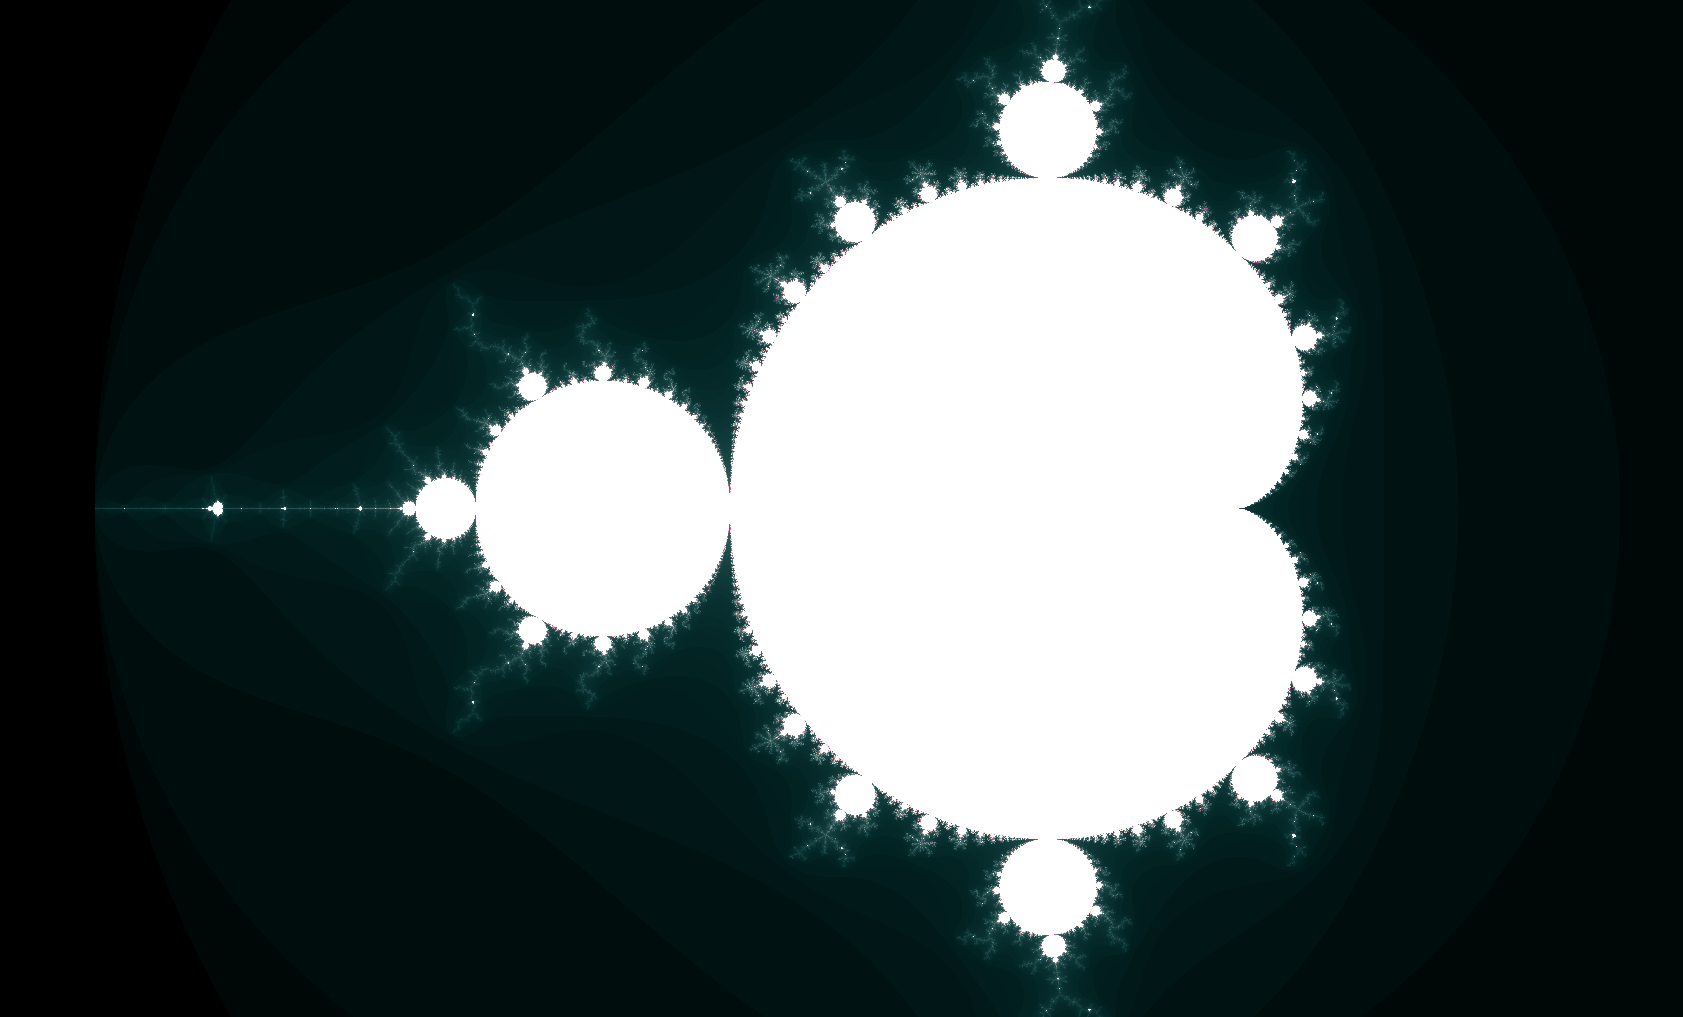
\includegraphics[width=0.65\linewidth, frame]{Images/Mandelbrot-2D-Full.png}
	\caption{The Mandelbrot set. The white points in the centre are inside the set.}
	\label{figure:mandelbrot-2d-full}
\end{figure}

The Mandelbrot set is the set of two-dimensional points that satisfy a certain constraint on the following complex quadratic equation:

\begin{equation} \label{equation:mandelbrot-2d}
	Z = {Z^2} + C
\end{equation}

where Z and C are complex numbers. The constraint on the points is that their orbit must be bounded. The value of Z is initialized to 0 and equation \ref{equation:mandelbrot-2d} is iterated over, each new value of Z being placed back in to the equation in the next iteration. If the length of the point Z does not exceed a threshold, then the point (represented by C) is in the Mandelbrot set \cite{devaney1999mandelbrot}.\newline

Figure \ref{figure:mandelbrot-2d-full} shows a generated Mandelbrot set. The real part of the point C is represented by the x-axis, and the imaginary part by the y-axis. Equation \ref{equation:mandelbrot-2d} is iterated over a maximum of five hundred times, and the threshold value is two. The pixels are coloured according to how many iterations are achieved before the length of Z exceeds the threshold.

\newpage

\begin{figure} [ht]
	\centering
	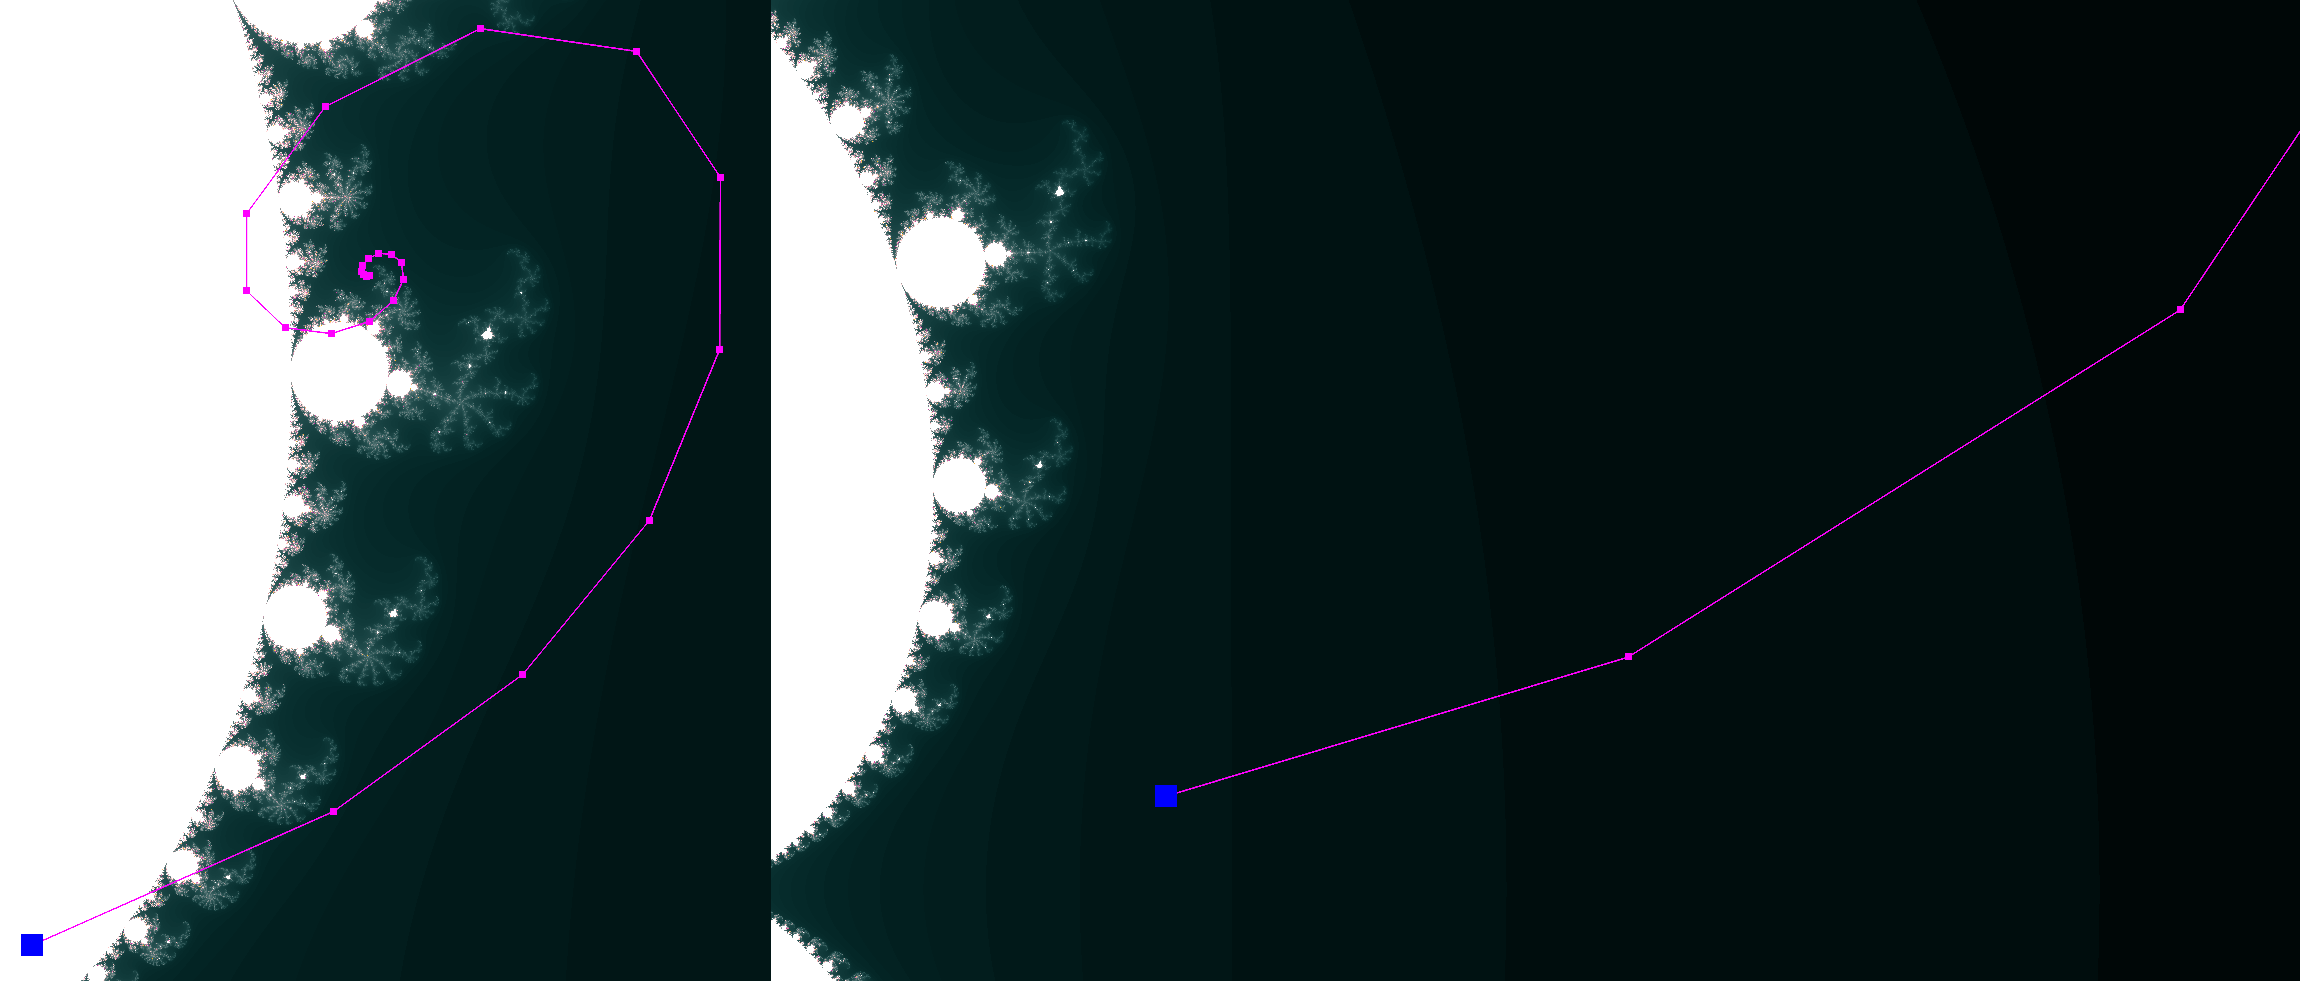
\includegraphics[width=\linewidth, frame]{Images/Mandelbrot-2D-Iterations.png}
	\caption{Visualization of the first twenty five iterations of equation \ref{equation:mandelbrot-2d} on the initial points [0.3, 0.05] (left) and [0.5, 0.04] (right). The initial points are shown in blue.}
	\label{figure:mandelbrot-2d-iterations}
\end{figure}

\begin{figure} [ht]
	\centering
	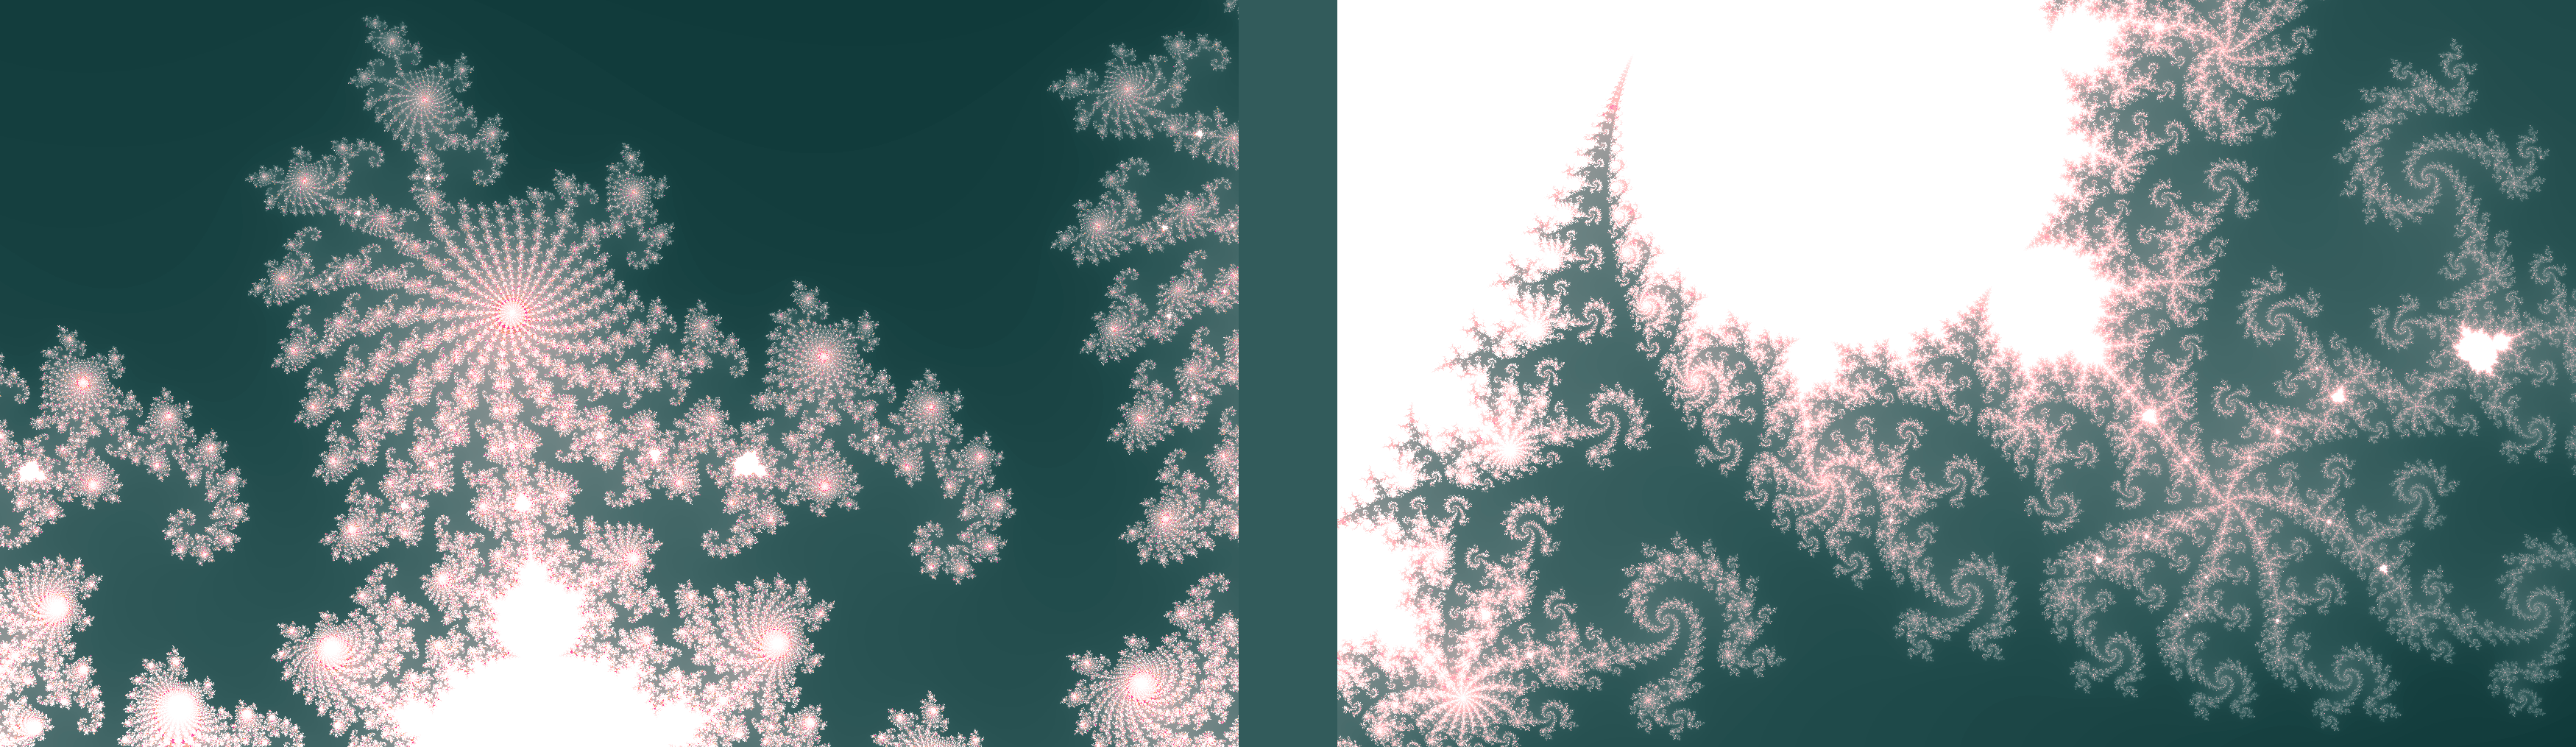
\includegraphics[width=\linewidth, frame]{Images/Mandelbrot-2D-Zoom.png}
	\caption{Two different views of the Mandelbrot set, zoomed in.}
	\label{figure:mandelbrot-2d-zoom}
\end{figure}

Figure \ref{figure:mandelbrot-2d-iterations} illustrates the first twenty five iterations on two different points. For the first point, the iterations converge in a spiral shape and the length of Z never exceeds the threshold of two, therefore the point is in the Mandelbrot set and is coloured white. For the second point, the iterations diverge and exceed the threshold of two within a few iterations, so this point is not in the Mandelbrot set and is coloured dark.\newline

Figure \ref{figure:mandelbrot-2d-zoom} shows two zoomed-in views at the edge of the original shape. New patterns can be seen, as well as repeated ones, and even new instances of the original shape. This is because the Mandelbrot set has infinite detail, so if one decreases the range of the axes, new patterns will emerge \cite{ashlock2006evolutionary}.\newline

This project makes use of three-dimensional fractal rendering, so the next section will look at the challenge of bringing this infinite level of detail to three dimensions.

\newpage

\section{3D Fractals - The Mandelbulb}

\begin{figure} [ht]
	\centering
	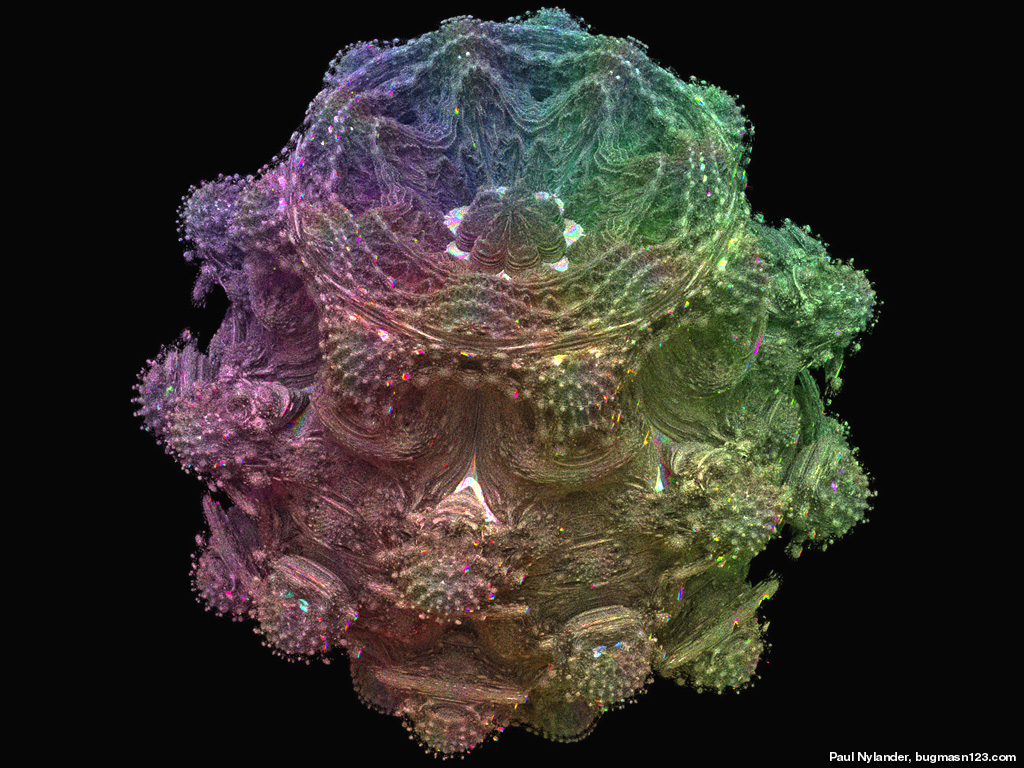
\includegraphics[width=0.5\linewidth, frame]{Images/Mandelbulb-First-Look.jpg}
	\caption{First look at the Mandelbulb, from Paul Nylander's website \cite{nylander-mandelbulb-image}.}
	\label{figure:mandelbulb-first-look}
\end{figure}

Since the Mandelbrot set is in two dimensions, and since complex numbers have only two components (real and imaginary), obtaining a true three-dimensional Mandelbrot set is a challenging task, and a mathematically rigorous three-dimensional Mandelbrot has not yet been found \cite{aron2009mandelbulb}.\newline

One attempt that seems to have come close was originated by Rudy Rucker in 1987. Rucker thought that expressing the three-dimensional points in spherical coordinates would allow the manipulation of the points in a similar way to the complex-number operations performed on the points in the two-dimensional Mandelbrot set \cite{rucker2009search}.\newline

Rucker did not have the computational power to accomplish a rendering of this idea, so it was put aside for twenty years, until Daniel White independently published a formula in 2007, which took the approach proposed by Rucker. White decided to approach the problem by considering the geometrical consequences of multiplying numbers in the complex plane, which amounts to rotating them \cite{aron2009mandelbulb}.\newline

White's formula produced images that looked promising, but they didn't have the level of detail that was expected from a true three-dimensional equivalent of the Mandelbrot set. A mathematician, Paul Nylander, raised White's formula to a higher power (eight), which would be equivalent to increasing the number of rotations of the point. The resulting image is shown in figure \ref{figure:mandelbulb-first-look}. The shape maintains excellent detail, even at high levels of magnification \cite {aron2009mandelbulb}.

\newpage

The new shape, known as the Mandelbulb, has roughly the same formula as the Mandelbrot set (equation \ref{equation:mandelbrot-2d}):

\begin{equation} \label{equation:mandelbulb}
	Z = {Z^k} + C
\end{equation}

where Z is raised to an arbitrary power like so:

\begin{equation} \label{equation:mandelbulb-power}
	{Z^k} = {r^k}(sin[k\theta]cos[k\phi], sin[k\theta]sin[k\phi], cos[k\theta]).
\end{equation}

The variable r is the norm of Z (|Z|), $\theta$ is equal to arctan($Z_y$/$Z_x$) and $\phi$ is equal to |($Z_x$, $Z_y$)|/$Z_z$. The spherical coordinates of the point Z/|Z| are represented by $\theta$ and $\phi$. Equations \ref{equation:mandelbulb} and \ref{equation:mandelbulb-power} are sourced from Chapter 33 of the book Ray Tracing Gems II \cite{marrs2021ray}.

\section{Signed Distance Functions}

Signed distance functions provide an estimate of how close a point is to the surface of a shape. If the result of the function is positive, then the point is outside the surface. If the result is negative, then the point is inside the surface. If the result is zero, then of course the point is exactly on the surface of the shape described by the function \cite{roblesprocedural}.\newline

A signed distance function can be derived using the B\"{o}ttcher map for the fractal formula, which is a deformation of the space. Closer to the surface of the fractal, the space is deformed to a greater degree than parts further away from the surface, as shown in figure \ref{figure:julia-bottcher-map}. The deformations of the space occur in such a way as to map the exterior of the fractal to the exterior of a unit disk \cite{quilez-distance}.\newline

A rigorous mathematical explanation of the B\"{o}ttcher map will not be given in this paper, but a brief introduction is helpful to understand the derivation of the distance function for the Mandelbulb. The map can be calculated as follows:

\begin{equation} \label{equation:bottcher-map}
	{\phi_C[Z]} = {lim_{n\rightarrow\infty}[f^n[Z]]^{k^{-n}}}
\end{equation}

where the value of f[Z] is the same as in equation \ref{equation:mandelbulb} and n refers to the current iteration of the equation \cite{marrs2021ray}.\newline

Looking at equation \ref{equation:bottcher-map}, take a point Z that is not in the fractal, so that the function f$^n$[Z] grows as the number of iterations increases, tending towards infinity. For a large enough value of n, the term f$_n$[Z] will become vastly larger than the value of C (as the point is far from the fractal), meaning that C can reasonably be discarded \cite{marrs2021ray}.

\newpage

\begin{figure} [ht]
	\centering
	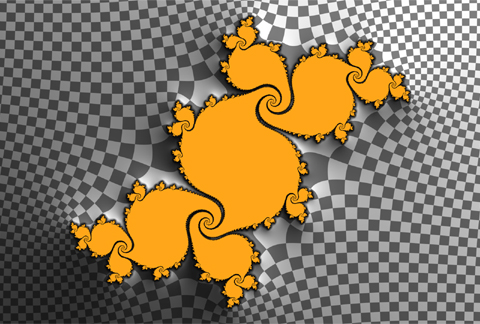
\includegraphics[width=0.5\linewidth, frame]{Images/Quilez-Bottcher-Map.jpg}
	\caption{The B\"{o}ttcher map generated for the Julia set (another two-dimensional complex fractal related to the Mandelbrot set), from the website of Inigo Quilez \cite{quilez-distance}.}
	\label{figure:julia-bottcher-map}
\end{figure}

From this casting away of C we obtain:

\begin{equation} \label{equation:mandelbulb-without-c}
	{f^{n+1}[Z] \approx {(f^n[Z])^k}}
\end{equation}

for points that are sufficiently far away from the surface of the fractal. Since the point at iteration n is far from the fractal, if one were to undo all of the iterations to get back to the original point at f$_0$[Z], we would obtain this expression:

\begin{equation} \label{equation:reverse-iterations}
	{{f_0^{n}[Z]}^{k^{-n}}} = Z
\end{equation}

and by extension, returning to the B\"{o}ttcher map:

\begin{equation} \label{equation:reverse-iterations-bottcher}
	\phi_0[Z] = Z
\end{equation}

which is the approximate result that equation \ref{equation:bottcher-map} gives when the function f$^n$[Z] ultimately diverges \cite{marrs2021ray}.\newline

Next, we will use something called the Hubbard-Douady potential, equal to the logarithm of the modulo of the B\"{o}ttcher map. This is a map of points onto a unit disk. Recall that the B\"{o}ttcher map maps the exterior of the fractal to the exterior of a unit disk. This now becomes important, as it enables us to use the Hubbard-Douady potential for all of our complex fractals. We now have a function that tends towards zero as the points approach the boundary of the fractal \cite{quilez-distance}:

\begin{equation} \label{equation:hubbard-douady}
	G[Z] = {lim_{n\rightarrow\infty}}\frac{log|{f^n}[Z]|}{k^n}.
\end{equation}

Equation \ref{equation:hubbard-douady} is not ready to be used as a distance measurement yet. However, it's possible to make it so. More detail is given in Ray Tracing Gems II, but a brief explanation will be given here. If we divide G[Z] by its gradient (obtaining this from the first-order Taylor expansion of the function), then we obtain an upper bound on the distance to the surface, which is desirable. The final equation for distance estimation therefore is \cite{marrs2021ray}:

\begin{equation} \label{equation:final-distance-estimate}
	d(Z) = {lim_{n\rightarrow\infty}}\frac{|f^n(Z)|log|f^n(Z)|}{|(f^n)'(Z)|}.
\end{equation}

\section{Ray and Sphere Tracing}

Ray tracing is a technique used for rendering scenes. Generally, a ray is a line that is cast from the camera or eye through each pixel of an image. Tests are performed to see which object (if any) is encountered by the ray first. By bouncing the ray from object to object, the program can gather the various light contributions from objects that reflect, emit or refract light \cite{haines2019ray}.\newline

Distance estimators can be used for ray tracing. If the approximate distance to the nearest surface can be calculated then the current point can be moved along the ray safely, until it is close enough to the surface to stop, according to this formula:

\begin{equation} \label{equation:sphere-tracing}
	{P_{n+1}} = {P_n} + \textbf{v}d({P_n})
\end{equation}

where P$_{n+1}$ is the point at the next step, P$_n$ is the point at the current step, \textbf{v} is the unit vector representing the ray direction and d(P$_n$) is the distance function acting on the current point \cite{marrs2021ray}.\newline

Using a distance function in this way is known as sphere tracing. The magnitude of the result of the distance function can be considered as the radius of a sphere. This sphere is guaranteed not to go through any part of the surface, making it safe to step according to the distance function result in any direction. For this guarantee to hold, the distance function must either be an exact calculation of the distance, or an underestimate \cite{hart1996sphere}.\newline

See figure \ref{figure:sphere-tracing}. This shows three scenarios for tracing a ray with the sphere tracing technique. At the bottom, the distance function is an exact measure of the distance to the nearest point on the surface. This is the ideal scenario, for correctness and performance. The top left image shows the result of a distance function which underestimates the distance each time. As a result, significantly more steps are taken along the ray, which will result in decreased performance. Lastly, the top right image shows the result of overestimating the distance. The ray ends up stepping past the boundary of the shape.

\newpage

\begin{figure} [ht]
	\centering
	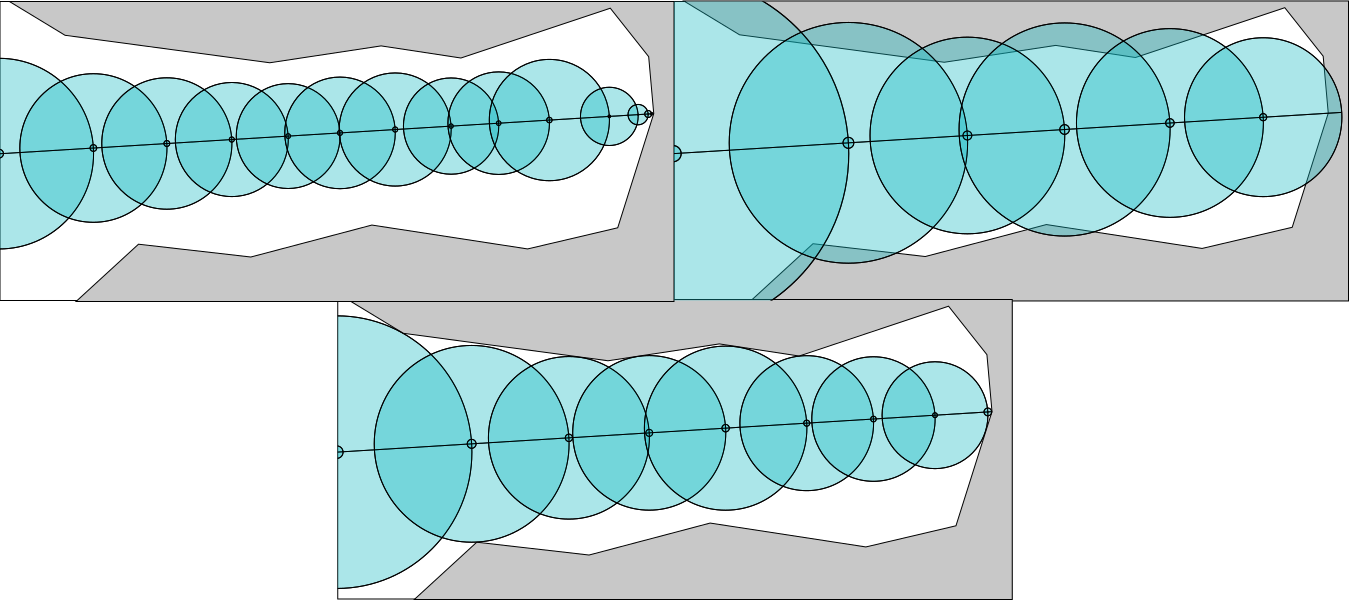
\includegraphics[width=0.75\linewidth, frame]{Images/Sphere-Tracing.png}
	\caption{Three scenarios in sphere tracing. Top left: Distance function underestimates distance, resulting in a loss of performance. Top right: Distance function overestimates distance, resulting in a loss of accuracy. Bottom: Distance function is exact.}
	\label{figure:sphere-tracing}
\end{figure}

\section{Signed Distance Fields}

Papers:
\begin{itemize}
	\item Signed distance fields: A natural representation for both mapping and planning \cite{oleynikova2016signed}.
	\item Hierarchical hp-adaptive signed distance fields \cite{koschier2016hierarchical}.
	\item Interactive ray tracing of distance fields (page 91) \cite{jamrivska2010interactive}.
\end{itemize}

- Stored values from signed distance function, stored as 2D texture or 3D grid.

- Saves having to recompute SDF all the time.

- Fractal scenes with high view distance could benefit from some pre-calculated values to give them a head start - show room of pillars and remark on frame rate (no SDF).

- Remark on memory costs.

- Briefly talk about storage methods - octrees.

- Talk about 2D methods - particularly used for fonts.

\section{Temporal Caching} \label{section:temporal-caching}

Papers:
\begin{itemize}
	\item Instant caching for interactive global illumination \cite{debattista2009instant}.
	\item Foveated real-time ray tracing for head-mounted displays \cite{weier2016foveated}.
\end{itemize}